%%%%%%%%%%%%%%%%%%%%%%%%%%%%%%%%%%%%%%%%%%%%%%%%%%%%%%%%%%%%%%%%%%%%%%%
%
%   Presentation of Beamer UMN Theme
   
%   Beamer Presentation by Tambe E. Norbert of UMN--Twin Cities
%  Hacked From Chris Bourke of Univ Nebraska--Lincoln
%  June 13th, 2014
%
%%%%%%%%%%%%%%%%%%%%%%%%%%%%%%%%%%%%%%%%%%%%%%%%%%%%%%%%%%%%%%%%%%%%%%%

\documentclass{beamer}

\usetheme[hideothersubsections,hideallsubsections]{UMNTheme}
% Remove navigation symbols
\setbeamertemplate{navigation symbols}{}

\title{Questions With GMSB MC}
\subtitle{}
\author{Tambe E. Norbert} %
\institute{University Of Minnesota}
\date{\today}

\begin{document}

%{% open a Local TeX Group
%\setbeamertemplate{sidebar}{}
\begin{frame}
        \titlepage
        \begin{center}
    \href{mailto:norbe072@umn.edu}{\color{blue}{\texttt{norbert@physics.umn.edu.edu}}}
        \end{center}
\end{frame}
%}% end Local TeX Group


\section{Neutralino Lifetime}

\begin{frame}
 %  \tableofcontents
   % \framesubtitle{}
  % \vspace{-1cm}
    \frametitle{Neutralino life time measurement}
    \begin{LARGE}  
  \textit{How are we measuring the neutralino Lifetime?}
    \end{LARGE}
    \begin{enumerate}
    \item Calculate time from distance travelled by Neutralino before it decays
       \begin{Definition}[Distance Travelled]
        \begin{displaymath}     
    \mathrm{L} = c\tau.\gamma \beta \quad \rightarrow  \quad c\tau = \frac{|\Delta\overrightarrow{r}|}{\gamma \beta}
    \end{displaymath}
    \end{Definition}
     \item 2 Extract time directly from MC
    \begin{Definition}[MC Time]
   \begin{displaymath}     
    c\tau = \frac{ct}{\gamma}
    \end{displaymath}
    \end{Definition}
       
    \end{enumerate}

    
\end{frame}


\section{Life Time Measurements}    

\begin{frame}
    \frametitle{ Neutralino Proper Decay length}
   % \framesubtitle{}
    \begin{figure}[ht]
    \begin{minipage}[b]{0.45\linewidth}
    \centering
     \mbox{
    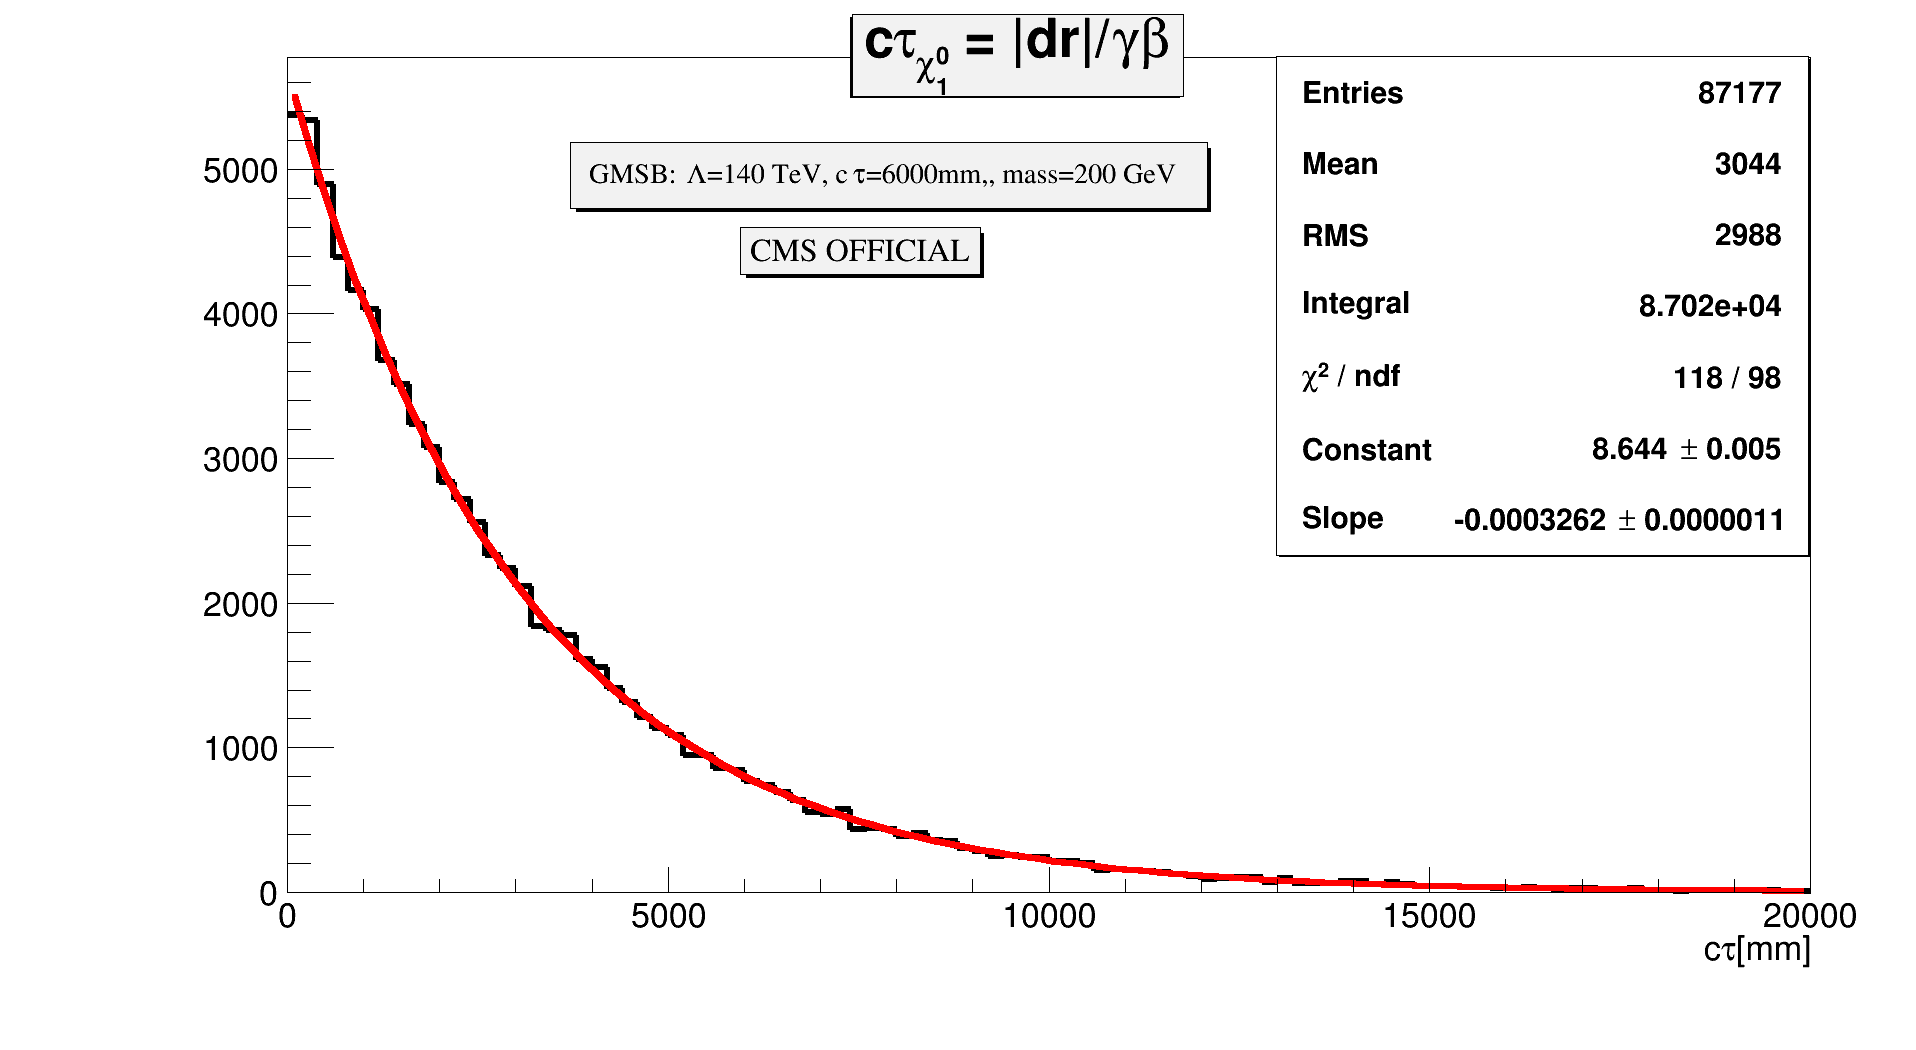
\includegraphics[height=6cm,width=\textwidth]{Dist_TravDL.png}}
    \vspace{-1cm}
     \caption{1/Slope = 3065.60 mm }
     \label{fig:Neutralino Distance}    
    \end{minipage}
    \hspace{0.1cm}
    \begin{minipage}[b]{0.45\linewidth}
    \centering
    \mbox{
    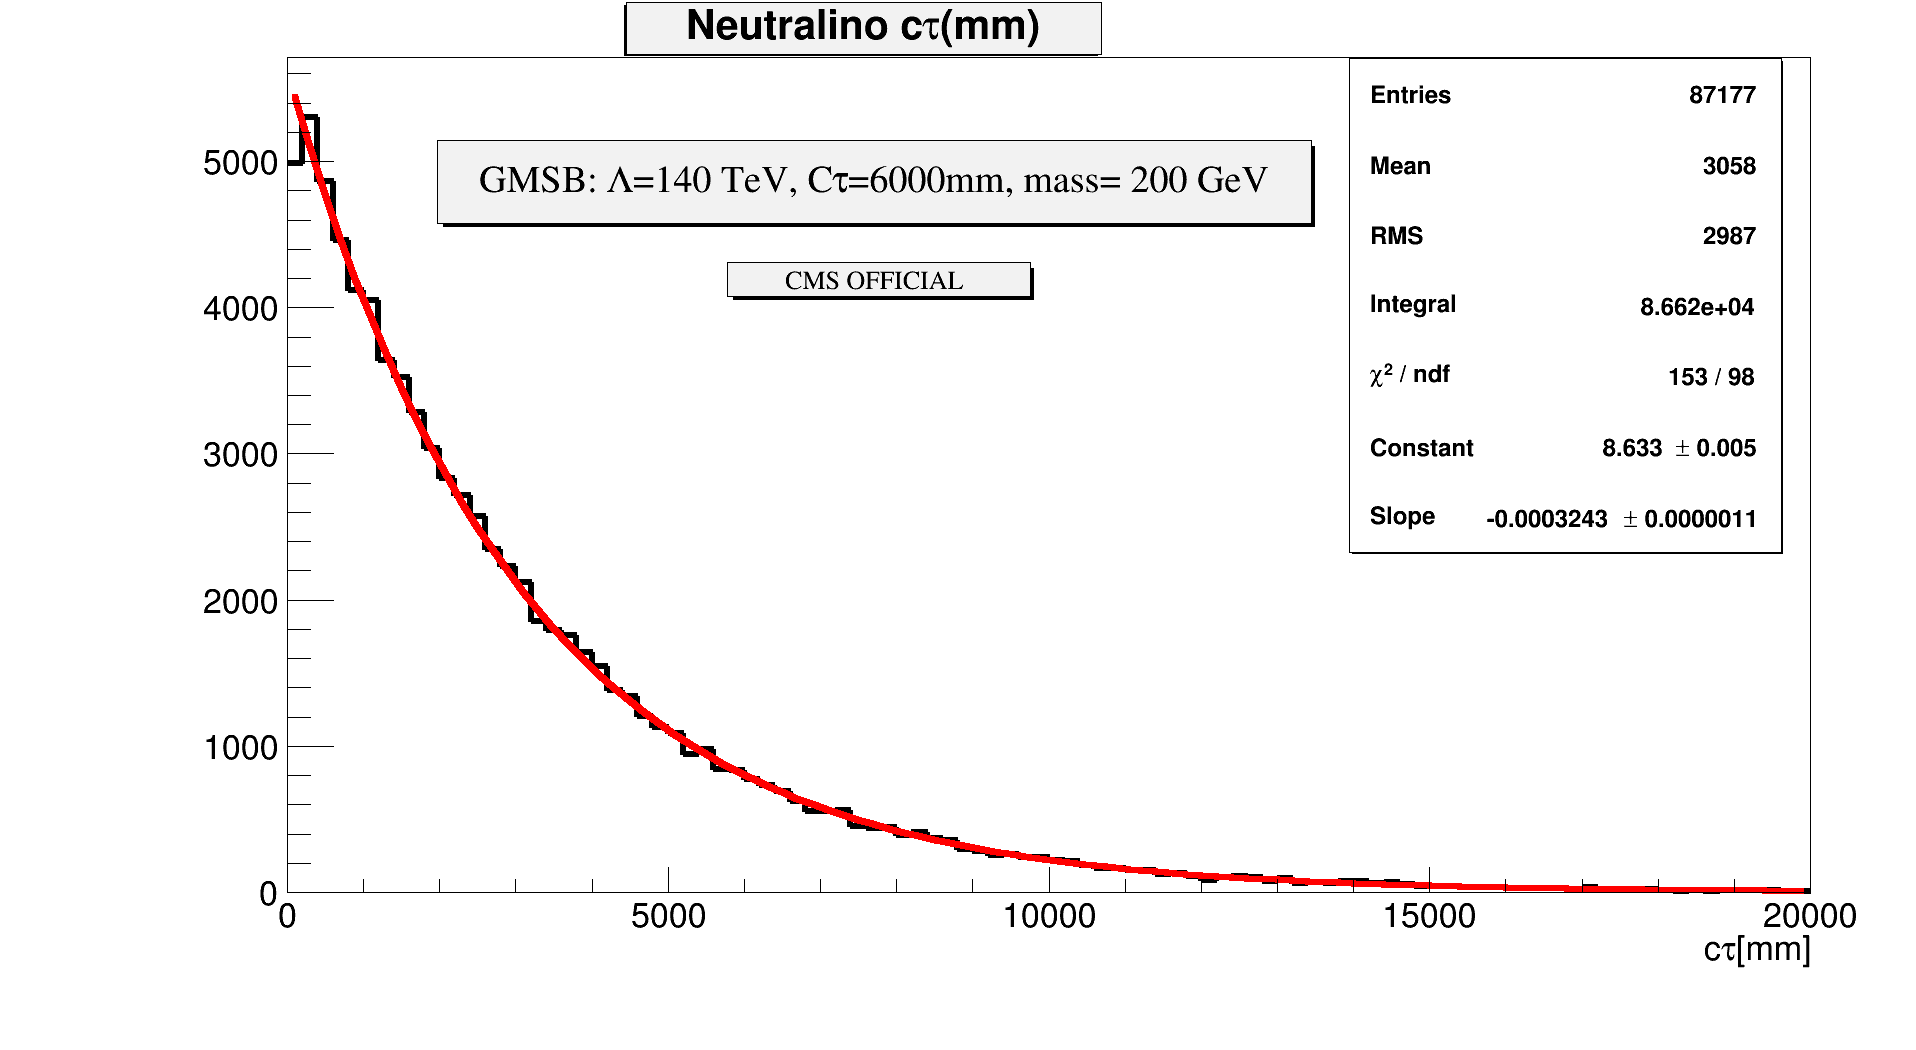
\includegraphics[height=6cm, width=\textwidth]{MC_TimeDL.png}}
     \vspace{-1cm}
    \caption{1/Slope = 3083.56 mm }
    \label{fig:From_MC}
     \end{minipage}
\end{figure}
\vspace{-1cm}
\alert{\textbf{Sample is $c\tau= 6000$ mm but we measure $c\tau \approx 3000$ mm}}

   
\end{frame}

\begin{frame}  %---------------------------------------------------------------
    \frametitle{Are these measurements correct?}
  %  \framesubtitle{}
  \begin{LARGE}  
  \textbf{Are we measuring the original $c\tau$  of the neutralino?}
    \end{LARGE}
    \vspace{-0.5cm}
\begin{table}
\begin{minipage}[b]{1.0\linewidth}
\centering
\begin{tabular}{|l||l||l||l|l|l|}
  \hline
  \multicolumn{5}{|c|}{\bfseries{CMS Official GMSB Samples}} \\
  \hline 
  \bfseries{$\Lambda$[TeV]} &  \bfseries{mass[GeV]} & \bfseries{$C_{grav}$} & \bfseries{c$\tau$[mm]} & \bfseries{Fit Value[mm]} \\
\hline  
120 & 169  & 93.5 & 1000 & 657.89 \\
120 & 169 & 162 & 3000  &1942.12 \\
\hline 
\hline
140 & 198 & 162 & 3000 & 1550.38 \\
140 & 198 & 187 & 4000 & 2064.83 \\
140 & 198 & 229 & 6000 & 3083.56 \\
\hline
\hline
180  & 256 & 93.5 & 1000 & 378.64 \\
180  & 256 & 132  & 2000 & 749.45 \\
180  & 256 & 162  & 3000 & 1104.85 \\
180 & 256 & 229 & 6000 & 2203.61 \\
\hline
  \end{tabular}
  \end{minipage}
\end{table}
\vspace{-0.5cm}
 \alert{\textbf{We seem to be measuring neutralino $c\tau$ by some factor off.}}
 
\end{frame}

\begin{frame}
%--------------------------------------------------------------------
\frametitle{GMSB Sample $c\tau$ Vs Measured $c\tau$}
\begin{LARGE}  
  \textbf{By how much are we off in  neutralino $c\tau$ measurements?}
    \end{LARGE}
\begin{table}
\begin{minipage}[b]{1.0\linewidth}
\centering
\begin{tabular}{|l||l||l||l|}
  \hline
  \multicolumn{4}{|c|}{\bfseries{CMS Official GMSB Samples}} \\
  \hline 
  \bfseries{$\Lambda$[TeV]} & \bfseries{c$\tau$[mm]} & \bfseries{Fit Value[mm]} &\bfseries{Factor Off} \\
\hline
120 & 3000 & 1942.12 & 1.54 \\
140 & 3000 & 1550.38 & 1.93 \\
180 & 3000 & 1104.85 & 2.71 \\
\hline
\hline
140 & 6000 & 3083.56  & 1.9 \\
180 & 6000 & 2203..61  & 2.7 \\
\hline
  \end{tabular}
  \end{minipage}
\end{table}
\vspace{-0.5cm}

Factor is \alert{The SAME} for different neutralino $c\tau$ with same $\Lambda$ value. However, factor is \alert{NOT THE SAME} for the same $c\tau$ with different $\Lambda$ values.

\end{frame}

\begin{frame}
%---------------------------------------------------------------------
\frametitle{Cause of this difference in $c\tau$ values?}
\begin{LARGE}  
  \textbf{Is this due to how sample is generated?}
    \end{LARGE}
    \vspace{-0.3cm}
 \begin{figure}[ht]
    \begin{minipage}[b]{0.45\linewidth}
    \centering
    \mbox{
    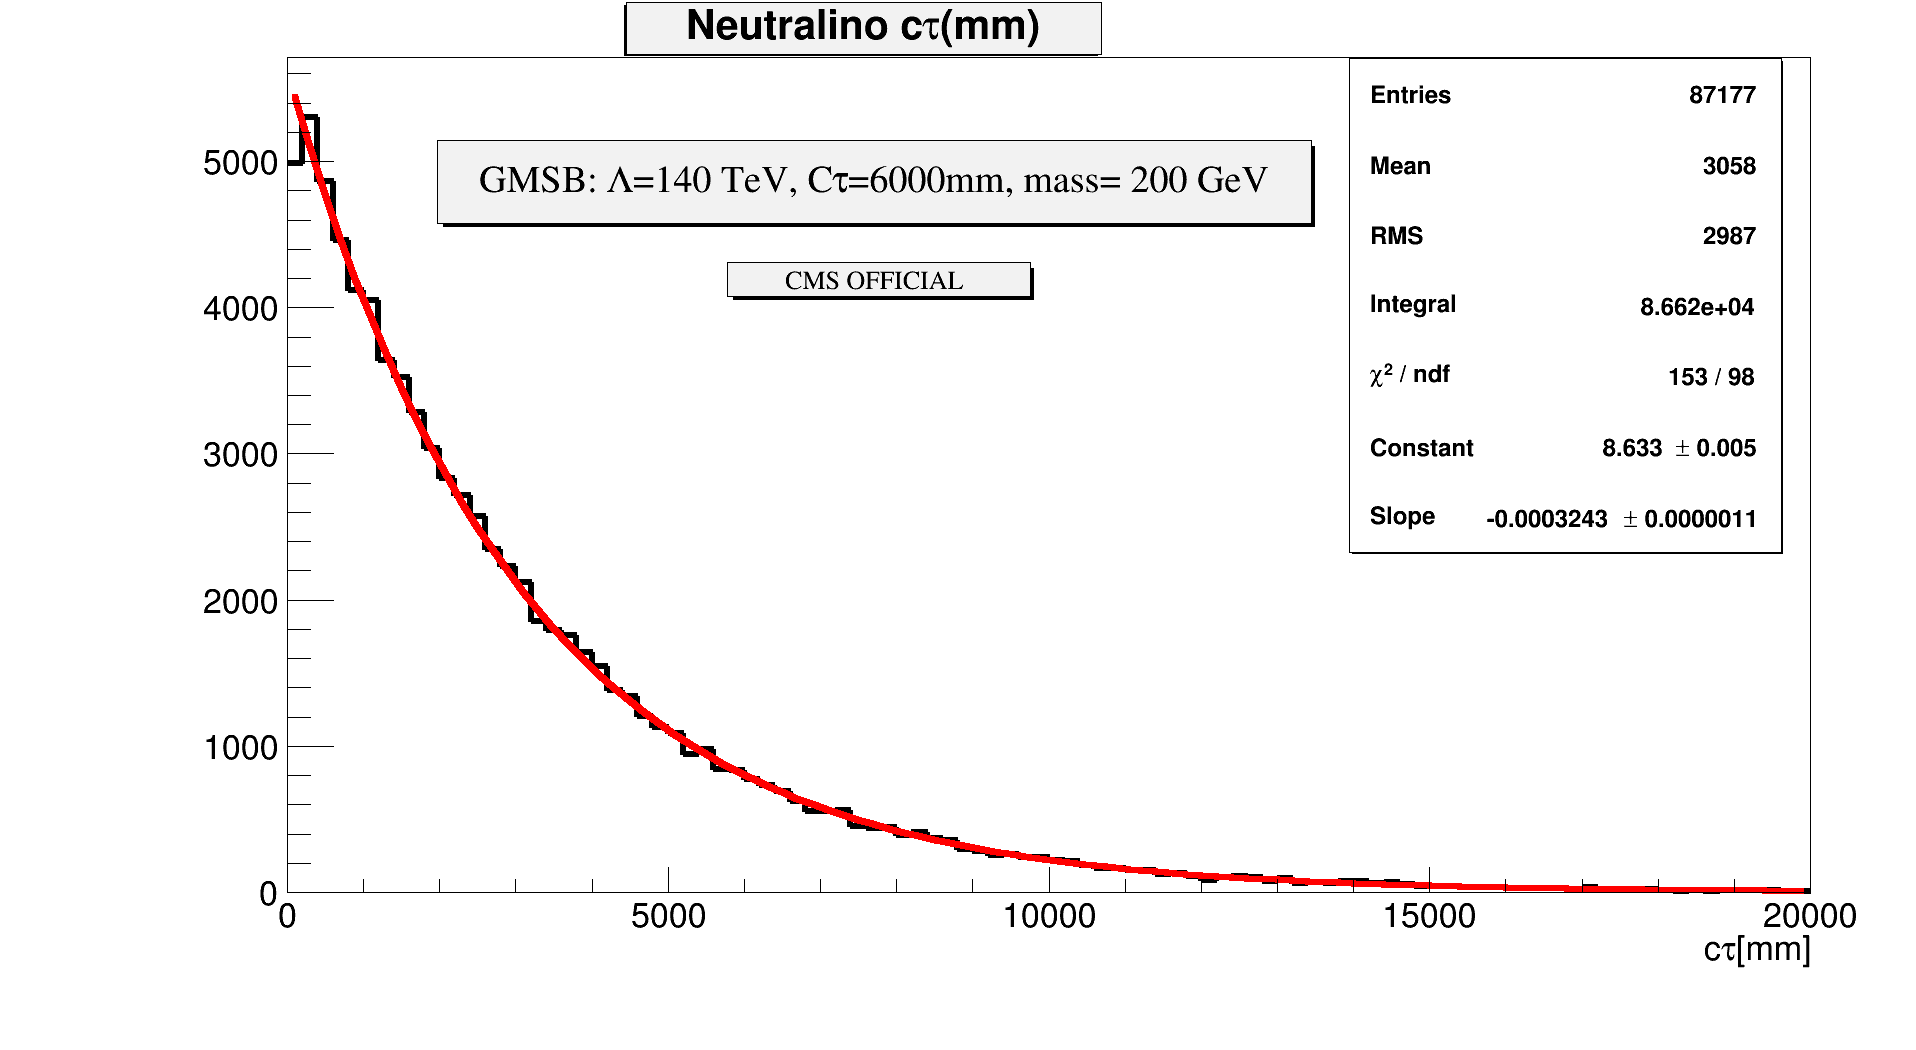
\includegraphics[height=2.5cm, width=\textwidth]{MC_TimeDL.png}}
     \vspace{-1cm}
    \caption{1/Slope = 3083.56 mm }
    \label{fig:OffFrom_MC}
    \end{minipage}
    \hspace{0.1cm}
    \begin{minipage}[b]{0.45\linewidth}
    \centering
    \mbox{
    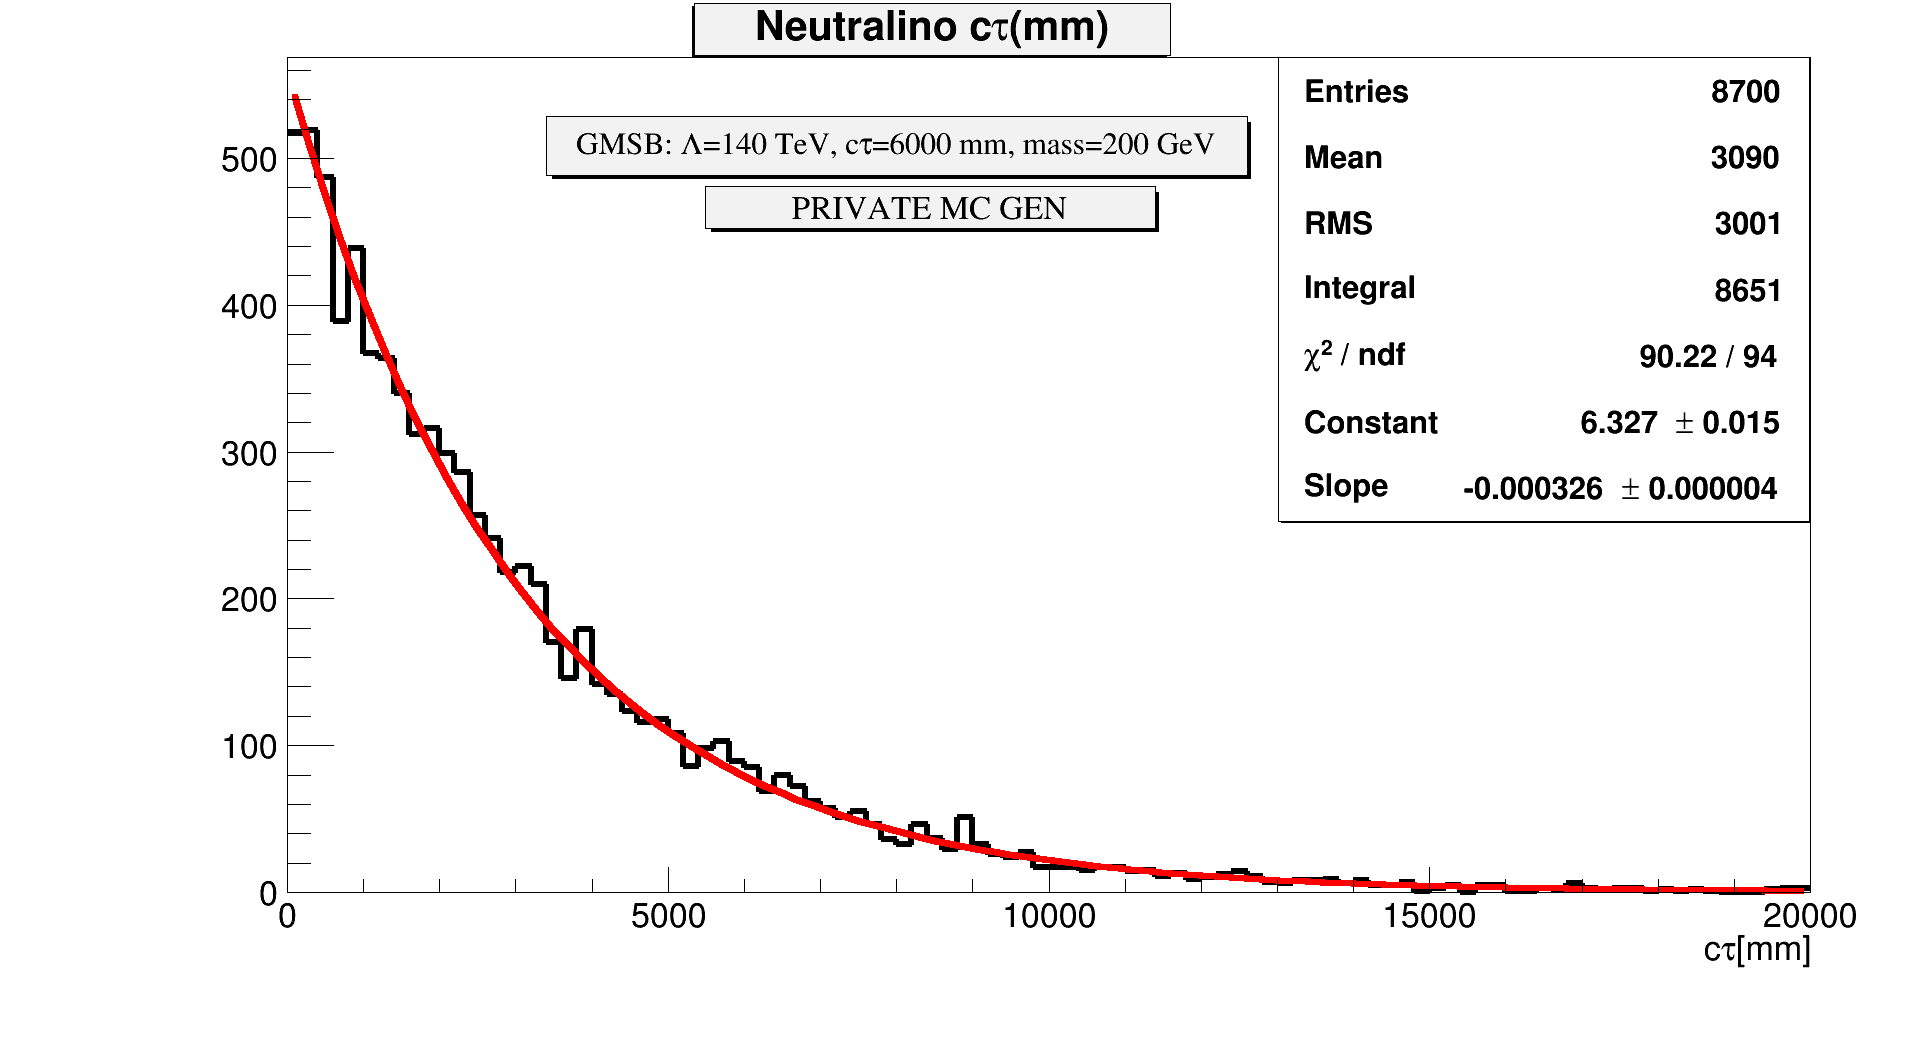
\includegraphics[height=2.5cm,width=\textwidth]{Priv_MC_TimeDL.png}}
    \vspace{-1cm}
     \caption{1/Slope = 3067.48 mm }
     \label{fig:Priv_MCTime}
     \end{minipage}
\end{figure}

\vspace{-1.0cm}

 \begin{figure}[ht]
    \begin{minipage}[b]{0.45\linewidth}
    \centering
    \mbox{
    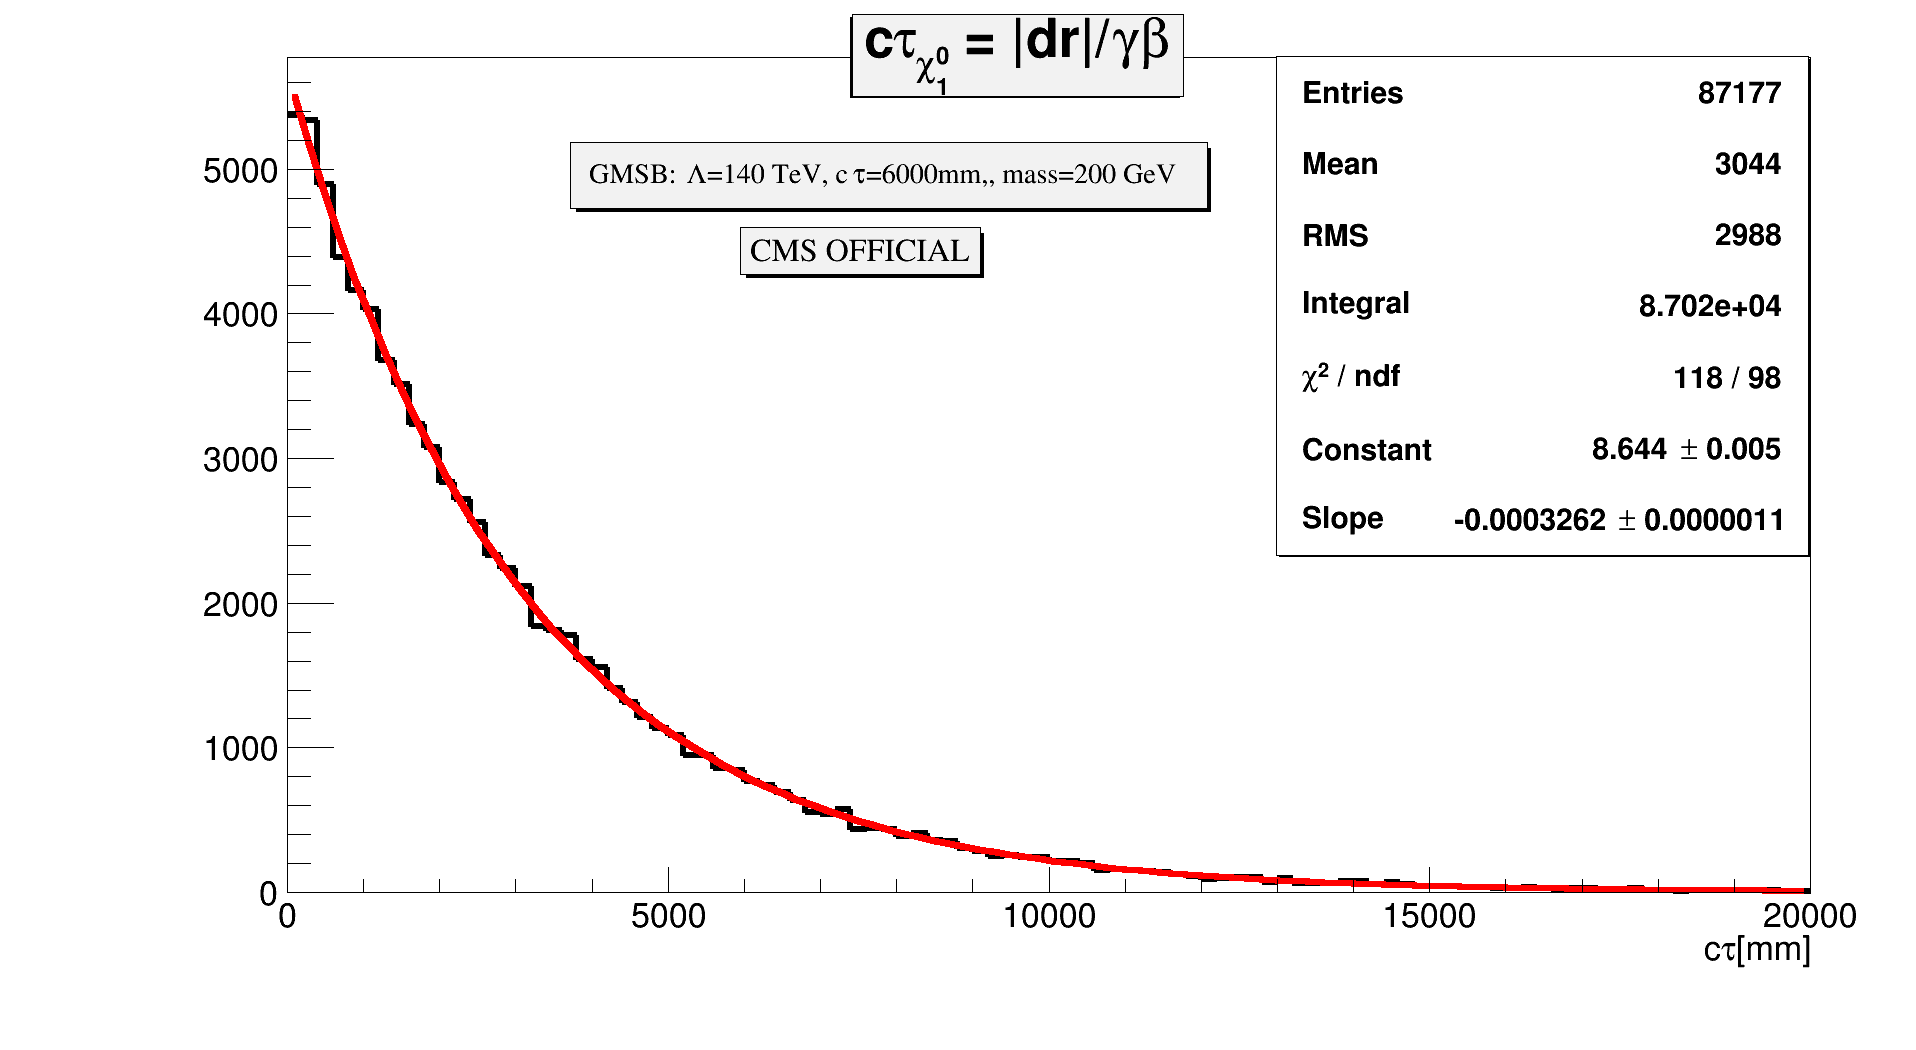
\includegraphics[height=2.5cm, width=\textwidth]{Dist_TravDL.png}}
     \vspace{-1cm}
    \caption{1/Slope = 3065.60 mm }
    \label{fig:Off_DL}
    \end{minipage}
    \hspace{0.1cm}
    \begin{minipage}[b]{0.45\linewidth}
    \centering
    \mbox{
    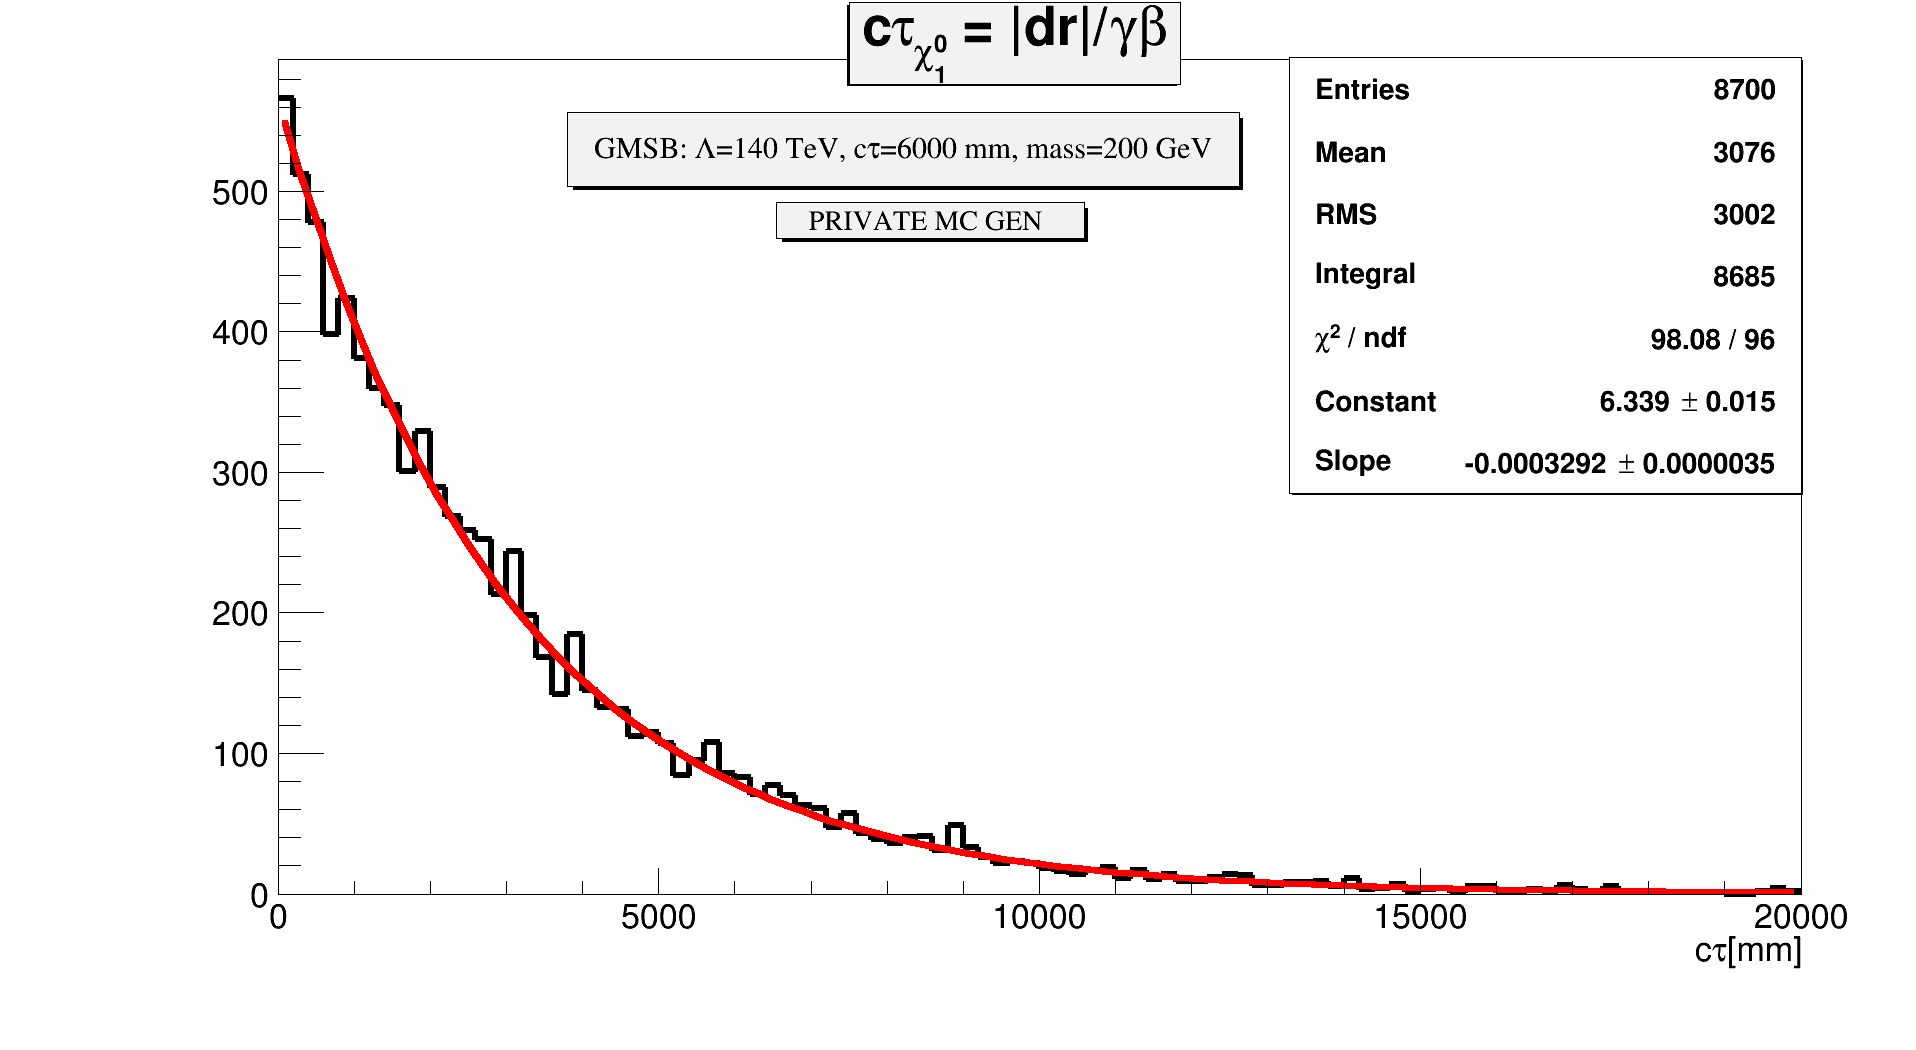
\includegraphics[height=2.5cm,width=\textwidth]{Priv_DistTravDL.png}}
    \vspace{-1cm}
     \caption{1/Slope = 3037.66 mm }
     \label{fig:Priv_DL}
     \end{minipage}
\end{figure}
\vspace{-1.0cm}
\alert{\textit{Private GMSB sample seems to show same offset measurements}}
\end{frame}




\begin{frame}
\section{Next Steps}
\frametitle{Origin Of $c\tau$ Difference?}
\begin{itemize}
\begin{large}
\item Offset in neutralino $c\tau$ seems to have a more subtle origin than expected. Probably how mass enters into the lifetime definition and implementation at MC generation level.
\item GMSB samples with the same sample $c\tau$, hence $C_{grav}$, but with different $\Lambda$ values have different offset factor.
\item The observation that the $c\tau$ value for a given sample with $\Lambda$ is different from the measured value is very unclear, even without looking at samples with different $\Lambda$ values.
\item Our next step involves understanding cause of this offset. 
%However,due to time constraints, we might continue with upper limit setting considering this difference.
\end{large}
\end{itemize}
\end{frame}
    
\end{document}